\documentclass[10pt,a4paper]{article}
\usepackage[utf8]{inputenc}
\usepackage{amsmath}
\usepackage{amsfonts}
\usepackage{amssymb}
\usepackage{tikz}
\usetikzlibrary{shapes, positioning, decorations.text}
\usepackage{wrapfig}

\begin{document}
\title{Trebuchet}
	\section{Optimum Release Angle}
		At what angle should a projectile be launched to achieve the greatest range?
		If the angle is too large the projectile will go very high but will not have much forward velocity.
		If the angle is too low the projectile will be moving forward very quickly but will not be in the air long enough to make it anywhere.
		What angle will balance these two scenarios and provide the optimum altitude with the best forward velocity?
		Do you have a guess? Think of throwing a ball. What angle do you use when you are trying to really get it to go far?
		Should we use that guess, or can we use our knowledge of math to \emph{prove} what will be the best angle?
		
		\begin{figure}
		\begin{tikzpicture}
			\draw[style=dashed] (0, 0) .. controls (2,3) and (6,3) .. (8, 0);
			\draw[->,ultra thick] (0,0)--(10,0) node[right]{$x$};
			\draw[->,ultra thick] (0,0)--(0,5) node[above]{$y$};
			\node[cross out, draw] at (8,0) {};
			\draw[->, thick] (0,0) -- (2,3) node[midway, above, sloped] (TextNode) {$V$};
			\draw (2,0) arc (0:56:2) node[pos=0.4, above] (TextNode) {\large{$\theta$}};
			\node at (8,-0.4) {$R$};
		\end{tikzpicture}
		\caption{What value of $\theta$ will produce the largest $R$?}
		\label{fig:launchAngle}
		\end{figure}
		
	\subsection{Breakup $V$ into its  X and Y Components}
		The first step is to break up our initial velocity vector $V$ into its two component vectors $V_x$ and $V_y$.
		This will tell us how fast our projectile is moving in these two directions.
		
		\begin{wrapfigure}{l}{0.45\textwidth}
		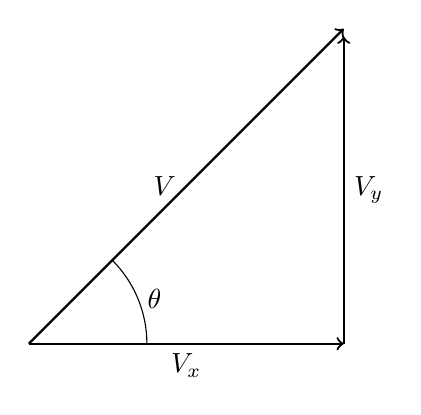
\begin{tikzpicture}
			\draw[->, thick] (0,0)--(4,0) node[below, midway] {$V_x$};
			\draw[->, thick] (4,0)--(4,3.9) node[right, midway] {$V_y$};
			\draw[->, thick] (0,0)--(4,4) node[left, midway] {$V$};
			\draw (1.5,0) arc (0:45:1.5) node[midway, right] {$\theta$};
		\end{tikzpicture}
		\caption{Component Vectors of $V$.}
		\label{fig:componentVectors}
		\end{wrapfigure}
		
		\noindent
		$V =$ launch velocity \\
		$\theta =$ launch angle \\
		$V_x =$ velocity in the $x$ direction \\
		$V_y =$ velocity in the $y$ direction \\
		
		How do we find the values of $V_x$ and $V_y$?
		Since we know that $V_x$ and $V_y$ form a right angle we can use the basic trig identities for $\sin, \cos, \tan$ to find the these values knowing only $V$ and $\theta$.
		
		$V_x = V \sin\theta$ \\
		$V_y = V \cos\theta$ \\
		
\end{document}